\documentclass[a4paper,11pt]{article}
\usepackage{xcolor}
\usepackage{geometry}
\usepackage{hyperref}
\hypersetup{
    colorlinks=false,
    linkcolor=blue,
    linkbordercolor=blue,
    pdfborderstyle={/S/U/W 1}
}
\usepackage{graphicx}
\usepackage{float}
\usepackage[strict]{changepage} %allows indented blocks
\usepackage{amsmath}
\geometry{
a4paper,
total={170mm,257mm},
left=20mm,
top=20mm,
marginparsep=0mm,
}
\setlength\parindent{0pt} % get rid of the stupid indent

\title{Networks Cheatsheet}
\author{Thomas Boxall\\ \texttt{up2108121@myport.ac.uk}}
\date{May 2023}

\usepackage{fancyhdr}
\pagestyle{fancy}
\fancyhead{} % clear all header fields
\renewcommand{\headrulewidth}{0pt} % no line in header area
\fancyfoot{} % clear all footer fields
\renewcommand{\footrulewidth}{0.4pt}
\fancyfoot[C]{\thepage} % page number in centre of the page
\fancyfoot[R]{\footnotesize Thomas Boxall\\ \texttt{up2108121@myport.ac.uk}} % right hand footer has author name on top line and author contact on bottom line
\fancyfoot[L]{\footnotesize Networks \\ May 2023} % left hand footer has title of document on top line and date on bottom line


\begin{document}

\maketitle
\thispagestyle{fancy}

\section{Protocols}
\textbf{Protocol} is a standard method or format for communication between network devices.\\
\textbf{What-If? Conditions} are covered by protocols. Protocols allow smooth recovery from if something goes wrong (e.g. What if a packet gets corrupt? What if the communication medium fails?)\\
\textbf{Connection Oriented Protocols} operate on connections which use virtual circuits which work like a old-style landline telephone where a dedicated connection between sender and receiver is established for the duration of the transmission then torn down after the transmission is complete. This provides a good Quality of Service (QoS) however they take time to setup and teardown, and while in use no other transmission are able to use that communication link.\\
\textbf{Connectionless Protocols} operate on general transmission mediums, a bit like how the postal system works (letters/ packets move from sorting office to sorting office/ switch or router to switch or router until it arrives at the destination). The sender sends the data to transmit into the network and hopes it arrives at the receiver. These are much more efficient than connection-oriented which makes them better for situations where the throughput of data is very important (e.g. audio/ video). However, the packets may get lost, or all go different routes and arrive in the wrong order - TCP is used here to solve this.\\
\textbf{TCP/IP} (Transmission Control Protocol/ Internet Protocol) is a collection of protocols that control how data travels from one machine to another across networks.
\begin{adjustwidth}{2em}{1em}
\textit{TCP} is connection-oriented and ensures reliable data delivery through sequencing, checksum and provides flow control. At the sending device, TCP breaks the data to send into packets which the network can handle then at the recipient, TCP examines all the packets to ensure they have all arrived and are all un-corrupt then reports the status back to the sender node so it knows if it needs to retransmit any of them, finally it will reassemble the packets into the data.\\
\textit{IP} is used to envelope the data, providing a location where the sender and destination IP addresses can be added to the packet.
\end{adjustwidth}
\textbf{UDP} (User Datagram Protocol) is a connectionless transport service (there is no guarantee the packets will arrive), it provides no error checking or sequencing. UDP is much more efficient than TCP.\\
\textbf{CSMA/CD} (Carrier Sense Multi Access/ Collision Detection) is an algorithm used on Bus Topologies which detects collisions and determines how to recover from them. The way it works can be seen in Figure \ref*{fig:csmacd}. 

\begin{figure}[ht]
    \centering
    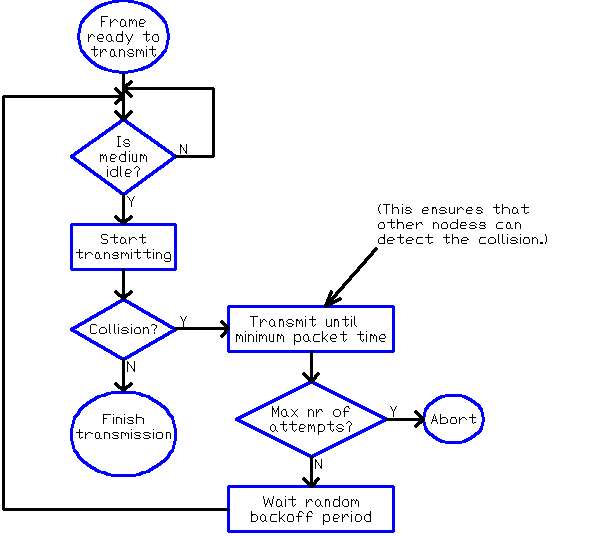
\includegraphics[width=0.8\textwidth]{../assets/csmacd.png}
    \caption{CSMA/CD Algorithm}
    \label{fig:csmacd}
\end{figure}

\section{Packets}
\textbf{Packets} are single units of data to be sent across a network. Data to be transmitted is broken into multiple packets.\\
\textbf{Packet Headers} contain the sender and recipient IP addresses.\\
\textbf{Routes} the packets takes are determined by routers. They control where the packet ``hops''. 

\section{Internet Protocol}
\textbf{Internet Protocol} (IP) is a connectionless protocol with best-effort delivery. It uses IP addresses.\\
\textbf{IP Address} is an identifier used to identify individual computers. They can either be statically assigned or dynamically assigned (this is done through DHCP) to a device.\\
\textbf{Subnet Mask} of an IP address is a 32-bit pattern used to identify the network and host address. Devices can have the same subnet mask as each other.\\
\textbf{IPv4} is the `original' format of IP addresses. It uses 32 bits.\\
\textbf{IPv6} is the `new' format of IP addresses as there were not enough in IPv4 for all devices. It uses 128 bits. 

\section{Network Capacity}
\textbf{Bandwidth} is the maximum rate of data transfer across a given path.\\
\textbf{Data rate} can be calculated using the following formula:
\begin{align*}
\mathrm{data\ rate\ (bytes/s)} &= \frac{1}{\mathrm{time\ interval\ of\ packet\ being\ sent}} \times \mathrm{packet\ size\ (bytes)}\\
\mathrm{data\ rate\ (bits/s)} &= \frac{\mathrm{data\ rate\ (bytes/s)}}{8}\\
\mathrm{data\ rate\ (kilobits/s)} &= \frac{\mathrm{data\ rate\ (bits/s)}}{1000}\\
\end{align*}

\section{Interconnection Components}
\textbf{Switches} examine the header of the packet as it arrives into the switch. The packet is forwarded to only the next node in its journey (this may be multiple places, in which case multicast is used). Switches can either operate in store and forward (where they temporarily hold the frame while making the decision about its destination) or cut through (where they start to forward the frame as soon as the destination IP address is read - requires switch and device to have same data rate).\\
\textbf{Hubs} transmit the packets to all of the connected devices, even if the packet isn't destined for that device. It is up to the device to check the recipient IP address and if it doesn't match its then the packet gets discarded.\\
\textbf{VLAN} (Virtual Local Area Network) are software which virtually divides a LAN into smaller LANs. Membership of a VLAN is set by the network admin and can be based off of which port on a switch the device connects to, MAC addresses, or a Layer 3 protocol (e.g. IP or IPX). 

\section{Standards}
\textbf{Standards} are documented agreements containing technical specifications or other precise criteria that stipulate how a particular product or service should be designed or performed. They exist outside of networking too.\\
\textbf{Standardisation Bodies} are the organisations which produce standards. Examples include IEEE (LAN standards), IEFT (Internet RFCs), ETSI (Eurpoean Telecoms), EIA/TIA (Cable standards i.e. CAT5/5e), ITU-T (Telecom \& data comms standards).  

\section{OSI Reference Model}
\textbf{Overview} The Open Systems Interconnection (OSI) reference model is based on a series of 7 layers. The data to be transmitted travels down through the seven layers to the transmission medium where it crosses the transmission medium and on the receiving device, the data climbs back up the seven layers.\\
\textbf{Layers} each have a specific function/ task. They each provide a service to the layer above. The four lower layers are concerned with the flow of data from end to end. The upper four layers are focused more towards services to the application. Layer 1 is closest to the transmission medium and layer 7 is closest to the application.
\begin{adjustwidth}{2em}{1em} 
\textit{Layer 1: Physical} is concerned with the physical characteristics of the transmission medium. It deals with voltage levels, timing of voltage changes, physical data rates, maximum transmission distances and physical connectors.\\
\textit{Layer 2: Data Link} provides access to the networking media and physical layer. It handles the transmission of the data across the medium to the intended destination. It uses MAC addresses to identify different stations on the same medium. It is concerned with network topology, network access, error notification, ordered delivery of frames, flow control. Protocols used include Ethernet, frame relay and FDDI. \\
\textit{Layer 3: Network} is concerned with the end-to-end delivery of packets. It defines the logical address \& how routing works. It also defines how to fragment packets into smaller packets to accommodate different media and its where routers operate.\\
\textit{Layer 4: Transport} regulates information flow to ensure end-to-end connectivity between host applications is reliable and accurate. TCP and UDP operate here.\\
\textit{Layer 5: Session} defines how to start, control and end sessions between applications using dialogue controls for multiple bi-directional messages. It synchronises dialogue between the two host's presentations layers and manages their data exchange as well as supporting efficient data transfer.\\
\textit{Layer 6: Presentation} ensures data is in common formats, provides encryption and compression of data. This is to ensure the data is readable by all devices.\\
\textit{Layer 7: Application} provides network services to the users applications. It checks the availability of intended communication partners and synchronises \& establishes agreement on procedures for error recovery and control of data integrity.
\end{adjustwidth}
\section{Communication Media}
\textbf{Wired approaches} involve networking cabinets which distribute the connection through wires to workstations.\\
\textbf{Wireless approach} involves a device broadcasting the signal wirelessly which devices can use to send and receive data.
\subsection{Wired Approach}
\textbf{Considerations} for designing a wired network should include: the required data rate (and what this might grow to in the future), the level of electrical interference, the maximum cable length, and finally the cost.\\
\textbf{Unshielded Twisted Pair} (UTP) Cables are a family a family of cables which will be found in most installations today. They are capable of working distances \textit{upto 100m}. 
\begin{itemize}
    \item Cat. 3 - to 10 Mbit/s or more
    \item Cat. 4 - to 20 Mbit/s or more
    \item Cat. 5 - to 100 Mbit/s or more
    \item Cat. 5e, 6 and 6A  - to 1000 Mbit/s and above (these are used extensively today)
\end{itemize}
\textbf{Cat. 6} adds additional quality assurances beyond Cat. 5e in that it comes in an additional form: \textit{Screened Twisted Pair (ScTP)} which has a layer of metallic foil to improve its interference rejection\\
\textbf{Shielded Twisted Pair} (STP) Cables were primarily used by IBM and should be better than UTP because it has a shield which helps prevent interference from outside signals and also helps prevent interference to outside signals. These are used extensively in \textit{Token Ring Topologies}. \\
\textbf{Coaxial Cable} produces very low amounts of noise therefore has a low bit-error rate. It is found in a variety of networking applications and its shielding may include multiple layers of foil or braid.\\
\textbf{Fibre-Optic Cable} have high data rates (100 Mbit/s in LAN or 1000 Mbit/s in telephone company links). Typically used in unidirectional mode (therefore deployed in pairs so there is one for each direction). They use light to transmit so electrical signal has to be converted to light and vice versa at the ends. Come in two forms: single mode (transmits single signal) which has internal diameter of $9\mu m$, and multimode (transmits multiple signals in same direction) which has internal diameter of $62.5\mu m$ for American sizes or $50\mu m$ for European sizes (over time \& distance signals can disperse and become corrupt). External diameter are often $125\mu m$ and relationship between internal and external is expressed as \textit{internal/external}.

\section{WAN Technologies}
\textbf{Asynchronous Transfer Mode} (ATM) is a standard for telecommunications which operates at the data-link layer (layer 2).\\
\textbf{Transparent LAN Services} (TLS) is where a carrier bridges between your geographically separated LAN Segments.\\
\textbf{Frame Relay} is a connection oriented public switched service provided by the telecommunications company, operated at layer 2 and is defined by the ITU-T and ANSI.\\
\textbf{PPP} Point-To-Point Protocol\\
\textbf{MPLS} MultiProtocol Layer Switching
\subsection{ATM}
\textbf{Supports} the transfer of data within a range of guarantees for quality of services, and is a core protocol used it the SONET/SDH backbone.\\
\textbf{Segments} data to be transmitted into 48-octet chunks which is paired with a 5-octet header which totals a 53-octet transmission chunk.\\
\textbf{Layered Architecture} is present in ATM. Each location ATM is used in has its own ATM Adaptation Layer (AAL) which breaks down as follows:
\begin{adjustwidth}{2em}{1em}
\textit{Layer 1} is used for voice and video (where there is a constant bit rate)\\
\textit{Layer 2} is sued for compressed voice and video (where there is a variable bit rate)\\
\textit{Layers 3 and 4} are used for general user data (unspecified bit rate)\\
\textit{Layer 5} is used for TCP/IP (unspecified bit rate)
\end{adjustwidth}
\textbf{Quality of Service} can be configured at each ATM interface. This allows us to set a \textit{Constant Bit Rate} which has a \textit{Peak Cell Rate} that can be sustained for a maximum interval before being problematic. Alternatively, a \textit{Variable Bit Rate} can be used which has a \textit{Sustainable Cell Rate} that can peak at a certain level. The \textit{Available Bit Rate} specifies a minimum guaranteed bit-rate and the \textit{Unspecific Bit Rate} will allocate traffic to all remaining transmission capacity.
\subsection{TLS}
\textbf{Carrier Bridges} are often ATM circuits (a good example of the heavy reliance on ATM by carriers.)\\
\textbf{Ethernet Access} to carrier's ATM networks is called `Metro Ethernet' or `Ethernet Transport' and is available in all Ethernet data rates. 
\subsection{Frame Relay}
\textbf{High Throughput} is provided through having larger frame sizes (1500+ bytes), having higher interface data rates and reducing processing requirements.\\
\textbf{Variation of High-Level Data Link Control} (HDLC) which detects and discards frames with errors, however doesn't retransmit them. A second protocol (e.g. TCP) which does this would be needed with Frame Relay.\\
\textbf{Two levels of traffic} are supported by Frame Relay. It has a \textit{Committed Information Rate} which all data up-to it will be accepted; and a \textit{Excess Information Rate} where between the CIR and EIR all data may be accepted however is marked as being `eligible for discard' with a reduction in cost.\\
\textbf{Congestion information} is transmitted with frame relay traffic. 

\section{Network Management}
\textbf{Motivation} for Network Management is to ensure as little downtime as possible - the more downtime, the greater the disruption to a business.\\
\textbf{Features} of network management include:
\begin{adjustwidth}{2em}{1em}
\textit{Configuration Management} is ensuring hardware devices are correctly configured which includes ensuring the assignments of network devices are correct, software is kept up to date and parameters are setup correctly.\\
\textit{Fault Management} provides identification and isolation of faults detected.\\
\textit{Performance Management} reviews statistical data generated from the network (e.g. round trip delays) and improving on those figures. This includes eliminating bottlenecks.\\
\textit{Accounting Management} is concerned with the billing of network usage which can include number of connections, capacity, number of emails, number of packets, amount of internet usage etc.\\
\textit{Security Management} includes confidentiality, integrity, authentication, access control and nonrepuditation.
\end{adjustwidth}

\section{Network Security}
\textbf{Security Problems} include: remote attacks, backdoors, insecure configuration, access controls, personal devices.\\
\textbf{Security Management} includes: control \& distribution of data, event logging, monitoring, parameter management.\\
\textbf{Security Services} include: denial of service prevention, access controls, user authentication, data confidentiality, and accountability. 

\end{document}